% =====================================================================
% Reformer digital twin -- manuscript for International Journal of Hydrogen Energy
% Overleaf: upload this file as main.tex and put the figure PDFs in a folder
% named "figures/". Compiler: pdfLaTeX. The bibliography is embedded, no .bib needed.
%
% LAYOUT OPTIONS (choose one; "3p" is the compact single-column journal layout)
%   final,3p,times            -> compact, single column, no line numbers   <-- active
%   final,5p,times,twocolumn  -> two-column journal look (wide tables need table*)
%   preprint,review,12pt      -> double spaced with line numbers, for referees
% To add line numbers for review, uncomment the two lineno lines below.
% =====================================================================
\documentclass[final,3p,times]{elsarticle}

\biboptions{numbers,sort&compress}

\usepackage{amsmath,amssymb}
\usepackage{graphicx}
\usepackage{booktabs}
\usepackage{xcolor}
\usepackage[hidelinks]{hyperref}
\hypersetup{pdfauthor={Madina Sissenbay and Izbassar Orynbassar},
            pdftitle={A physics-informed digital twin for tube-life-aware operation of industrial steam methane reformers under uncertainty}}
% \usepackage{lineno}   % uncomment this pair to number lines for review
% \linenumbers

\graphicspath{{figures/}}
\newcommand{\todo}[1]{\textcolor{red}{[TODO: #1]}}
\newcommand{\ce}[1]{\mathrm{#1}}

\journal{International Journal of Hydrogen Energy}

\begin{document}

\begin{frontmatter}

\title{A physics-informed digital twin for tube-life-aware operation of industrial steam methane reformers under uncertainty}

\author[au]{Madina Sissenbay}
\ead{m.sisenbay@aogu.edu.kz}
\ead[url]{https://orcid.org/0009-0009-8160-7472}
\author[su]{Izbassar Orynbassar\corref{cor1}}
\ead{iorynbas@syr.edu}
\ead[url]{https://orcid.org/0009-0002-4224-3249}
\cortext[cor1]{Corresponding author.}
\affiliation[au]{organization={Institute of Petrochemical Engineering and Ecology named after N.K. Nadirov,
  Safi Utebayev Atyrau University of Oil and Gas},
  city={Atyrau}, country={Kazakhstan}}
\affiliation[su]{organization={School of Information Studies, Syracuse University},
  addressline={343 Hinds Hall}, city={Syracuse}, postcode={13244}, state={NY}, country={USA}}

\begin{abstract}
Catalyst tubes are the life-limiting component of a steam methane reformer, yet operating decisions are rarely taken with a quantified tube-life cost. A digital twin is assembled from published data and open code, coupling a one-dimensional Xu--Froment tube model, a long-furnace model of a top-fired box furnace, a Larson--Miller creep-life module built on manufacturer rupture curves with their printed scatter band, and Gaussian-process surrogates with conformal prediction intervals. The tube model is verified against an industrial simulation, and the coupled model is calibrated on three published plant operating points with leave-one-case-out cross-validation, reproducing outlet temperatures within 4~K and tube-wall temperatures within 12~K. Firing intensity, steam-to-carbon ratio and excess air explain 82\,\% of the hot-spot temperature variance with negligible interactions. Under outlet-temperature control, load-following changes the tube-life cost per kmol of hydrogen by less than 2\,\% in either direction, whereas catalyst aging under a constant methane-slip target doubles it within four years. A Pareto knee delivers 15\,\% more hydrogen at 17\,\% less fuel per kmol for 0.28 of the base life cost, and creep-curve scatter dominates the life-prediction variance at 86\,\%. Regime rankings hold on four rupture curves; absolute lives do not.
\end{abstract}

\begin{highlights}
\item Open digital twin couples reformer kinetics, furnace, tube wall and creep life
\item Calibrated on published plant data: outlet T within 4 K, wall T within 12 K
\item Firing, steam-to-carbon and excess air govern hot-spot temperature and life
\item Catalyst aging doubles tube-life cost; load-following changes it under 2 \%
\item Creep-curve scatter dominates life uncertainty; regime rankings survive it
\end{highlights}

\begin{keyword}
steam methane reforming \sep digital twin \sep creep life \sep uncertainty quantification \sep multi-objective optimization \sep conformal prediction
\end{keyword}

\end{frontmatter}

% =====================================================================
\section{Introduction}
\label{sec:intro}

Steam methane reforming (SMR) supplies the large majority of the world's hydrogen, close to 100~Mt per year and still produced predominantly from natural gas without carbon capture~\cite{iea2024}; it will remain the dominant route for at least a decade while electrolytic capacity is built up. The core of an SMR plant is a top-fired or side-fired furnace in which several hundred centrifugally cast high-alloy tubes, filled with nickel catalyst, carry natural gas and steam at 25--35~bar while their outer walls are heated to 1100--1200~K. The tubes operate in the creep regime by design, and their remaining life is the single most important maintenance variable of the plant: a tube failure forces an unplanned shutdown, retubing costs about a tenth of the installed plant cost~\cite{latham2011}, and service life varies between 30\,000 and 180\,000~h with material quality and operating conditions~\cite{ray2003}. Tube life is governed almost entirely by the outer-wall temperature at the hottest elevation, because the rupture time roughly halves for every 10--20~K of additional metal temperature~\cite{latham2011,api530}; the rupture curve used here halves the life every 13~K at the stress of the calibrated tube.

Operating decisions therefore trade hydrogen production, fuel consumption and tube life against each other, but the trade-off is rarely quantified: plants are run against a maximum tube-wall temperature limit read from pyrometer surveys, and the effect of a load, steam-to-carbon or burner change on tube life is left to experience. Two developments make a quantitative approach both necessary and possible. Hydrogen plants are increasingly expected to follow variable downstream demand or to operate alongside intermittent electrolytic hydrogen, which raises the question of what tube life flexible operation costs; and validated models of the tube~\cite{xu1989a,xu1989b,pantoleontos2012,latham2011} and furnace~\cite{plehiers1989,zamaniyan2008} exist, surrogates make them fast enough for hourly simulation and optimization~\cite{kumar2015,jafarizadeh2024,yerimah2025,nabavi2025}, and rupture data for the relevant alloys are documented in public data sheets and manufacturers' design curves~\cite{nims16b,nims38a,yeh2021}. What is missing is a coupled, calibrated and uncertainty-aware chain from operating inputs to tube life, built entirely on published data and open code, so that its conclusions can be checked and its data replaced.

\subsection{Previous work}

The reformer tube has been modeled at every level of complexity. Xu and Froment~\cite{xu1989a} established the Langmuir--Hinshelwood--Hougen--Watson kinetics of methane steam reforming and water-gas shift on a Ni/MgAl$_2$O$_4$ catalyst that remains the standard intrinsic model, and in the companion paper~\cite{xu1989b} simulated an industrial tube with a one-dimensional heterogeneous model. The tube has since been coupled to a zone model of the furnace~\cite{plehiers1989}, to a unified top-fired model with three-dimensional zonal analysis~\cite{zamaniyan2008} and to a dynamic heterogeneous formulation~\cite{pantoleontos2012}. Latham and co-workers~\cite{latham2008,latham2011} calibrated a Hottel zone-method model of a top-fired box reformer on plant measurements including infrared tube-wall temperature surveys, and published the operating points and absolute tube-wall temperatures in the thesis appendix~\cite{latham2008}; that data set is the basis of the present calibration. Computational-fluid-dynamics models of the furnace~\cite{lao2016,tran2017,kumar2017} resolve the temperature field but are used to balance tube temperatures rather than to quantify life, and the data-driven work of the last decade --- furnace-balancing and smart-manufacturing frameworks~\cite{kumar2015,kumar2017,tran2017}, CFD-trained machine-learning surrogates~\cite{jafarizadeh2024,nabavi2025} and uncertainty-aware production optimization~\cite{yerimah2025} --- addresses production and efficiency: tube life, when it appears, enters as a constraint on a maximum temperature rather than as an objective with a quantified cost, and the uncertainty in kinetics, heat transfer and creep data is not propagated to the conclusions.

On the materials side, the creep behavior of the 25Cr--20Ni (HK40) and 25Cr--35Ni--Nb (HP-Nb) families of centrifugally cast tube alloys is characterized in the long-term data sheets of the National Institute for Materials Science~\cite{nims16b,nims38a,whittaker2013} and in remaining-life studies of service-exposed tubes~\cite{ray2003,haidemenopoulos2021,guguloth2023}. Yeh~\cite{yeh2021} combined a computed tube-wall temperature with a manufacturer's Larson--Miller curve for a proprietary HP-Nb alloy to estimate life, and showed that evaluating the life at the average instead of the maximum tube temperature overstates it by two orders of magnitude. The Larson--Miller parameter~\cite{larson1952} and the linear life-fraction rule of Robinson~\cite{robinson1952} remain the basis of design codes such as API~530~\cite{api530}.

\subsection{Contribution and research questions}

This paper presents a physics-informed digital twin of an industrial top-fired SMR linking operating inputs to tube creep life through the module chain of Fig.~\ref{fig:schematic}, verified against Xu and Froment~\cite{xu1989b}, calibrated on the plant data of Latham~\cite{latham2008}, and produced throughout by a versioned open pipeline from published data. Four research questions are answered:
\begin{description}
\item[RQ1] Which operating variables govern the hot-spot temperature and the creep-life consumption of the tube, and how do they interact?
\item[RQ2] What is the tube-life cost, per unit of hydrogen produced, of flexible operation (load-following, renewable-following, over-firing events) and of catalyst aging, relative to steady operation?
\item[RQ3] Which operating regimes are Pareto-optimal in hydrogen production, fuel consumption and life consumption, and how does the answer depend on how steam is charged?
\item[RQ4] How uncertain are these answers, which uncertainty sources dominate, and which conclusions survive the uncertainty?
\end{description}

% =====================================================================
\section{Methods}
\label{sec:methods}

\begin{figure}[t]
\centering
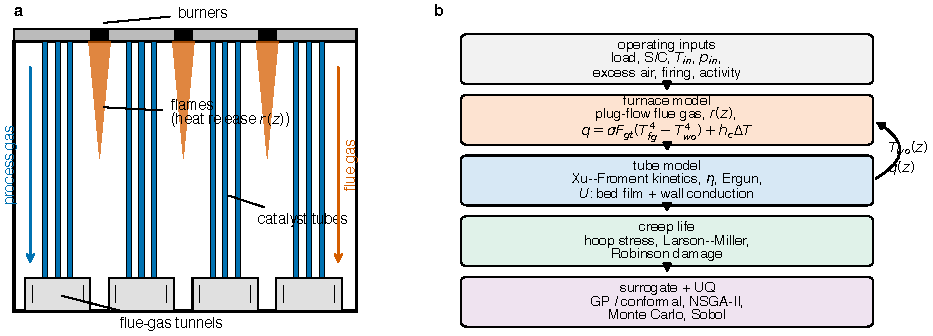
\includegraphics[width=\textwidth]{fig01_schematic}
\caption{(a) Cross-section of a top-fired box reformer: burners in the roof between rows of catalyst tubes, flames releasing heat in the upper part of the firebox, flue gas flowing downward co-currently with the process gas and leaving through tunnels at the floor. (b) Module chain of the digital twin: operating inputs are mapped through the furnace and tube models, which exchange the outer-wall temperature profile and the heat flux, to the creep-life module; surrogates and uncertainty quantification wrap the chain.}
\label{fig:schematic}
\end{figure}

The twin is implemented as a Python package (\texttt{rdt}) whose modules follow the chain of Fig.~\ref{fig:schematic}b. All physical data (kinetic parameters, plant operating points, creep curves) are read from annotated YAML and CSV files; no number is hard-coded in the model code. Thermodynamic properties, heat capacities and reaction equilibrium constants are taken from Cantera~\cite{cantera} with the GRI-Mech~3.0 species data, so that kinetics and energy balance are mutually consistent.

\subsection{Reactor tube model}
\label{sec:tube}

The tube is described by a steady one-dimensional pseudo-homogeneous plug-flow model with axial coordinate $z$ from the inlet (top) to the outlet. The state consists of the molar flows $F_i$ of CH$_4$, H$_2$O, H$_2$, CO, CO$_2$ and N$_2$, the process-gas temperature $T$ and the pressure $p$. The intrinsic kinetics are those of Xu and Froment~\cite{xu1989a} for steam reforming ($r_1$), water-gas shift ($r_2$) and overall reforming to CO$_2$ ($r_3$):
\begin{align}
r_1 &= \frac{k_1}{p_{\ce{H_2}}^{2.5}}\,\frac{p_{\ce{CH_4}}\,p_{\ce{H_2O}} - p_{\ce{H_2}}^{3}\,p_{\ce{CO}}/K_1}{\mathrm{DEN}^2}, \label{eq:r1}\\
r_2 &= \frac{k_2}{p_{\ce{H_2}}}\,\frac{p_{\ce{CO}}\,p_{\ce{H_2O}} - p_{\ce{H_2}}\,p_{\ce{CO_2}}/K_2}{\mathrm{DEN}^2}, \label{eq:r2}\\
r_3 &= \frac{k_3}{p_{\ce{H_2}}^{3.5}}\,\frac{p_{\ce{CH_4}}\,p_{\ce{H_2O}}^{2} - p_{\ce{H_2}}^{4}\,p_{\ce{CO_2}}/K_3}{\mathrm{DEN}^2}, \label{eq:r3}\\
\mathrm{DEN} &= 1 + K_{\ce{CO}}\,p_{\ce{CO}} + K_{\ce{H_2}}\,p_{\ce{H_2}} + K_{\ce{CH_4}}\,p_{\ce{CH_4}} + K_{\ce{H_2O}}\,p_{\ce{H_2O}}/p_{\ce{H_2}}, \label{eq:den}
\end{align}
with partial pressures in bar. The rate coefficients $k_j$ and adsorption constants $K_i$ follow the Arrhenius and van't~Hoff forms with the activation energies, adsorption enthalpies and reference values of Table~5 of~\cite{xu1989a}, reparameterised at the reference temperatures 648~K and 823~K used in that table so that the reported confidence intervals can be propagated directly (Section~\ref{sec:campaigns}). The equilibrium constants $K_1$--$K_3$ are computed from Gibbs energies of formation rather than from fitted expressions, which removes a source of inconsistency with the energy balance (Section~S1).

The balances per tube are
\begin{align}
\frac{\mathrm{d}F_i}{\mathrm{d}z} &= A_{\mathrm{cs}}\,\rho_b \sum_j \nu_{ij}\,\eta_j\,r_j, \label{eq:species}\\
\sum_i F_i c_{p,i}\,\frac{\mathrm{d}T}{\mathrm{d}z} &= \pi d_i\,U\,\big(T_{\mathrm{wo}}(z) - T\big) - A_{\mathrm{cs}}\,\rho_b \sum_j \eta_j\,r_j\,\Delta H_j(T), \label{eq:energy}\\
-\frac{\mathrm{d}p}{\mathrm{d}z} &= \frac{1-\phi}{\phi^3}\left(1.75 + 150\,\frac{1-\phi}{Re_p}\right)\frac{\rho_g v_s^2}{d_p}, \label{eq:ergun}
\end{align}
where $A_{\mathrm{cs}}$ is the cross-section, $\rho_b$ the bed density, $\eta_j$ the effectiveness factors, $\phi$ the bed voidage, $d_p$ the equivalent particle diameter and $Re_p$ the particle Reynolds number; Eq.~\eqref{eq:ergun} is the Ergun equation~\cite{ergun1952}. Rather than solving the pellet problem, constant effectiveness factors $\eta_j = 0.05$ in the first tenth of the tube and $0.1$ thereafter are used, and higher alkanes in the feed (C$_2$--C$_5$) are converted to CO and CH$_4$ at the inlet; both follow Latham et al.~\cite{latham2011} and are set out in Section~S1.

The overall heat-transfer coefficient referred to the inner surface combines the bed-side film coefficient $\alpha_i$ and the conduction through the tube wall,
\begin{equation}
\frac{1}{U} = \frac{1}{\alpha_i} + \frac{d_i}{2\lambda_t}\ln\frac{d_o}{d_i}, \qquad
T_{\mathrm{wi}} = T_{\mathrm{wo}} - q''_o\,\frac{d_o}{2\lambda_t}\ln\frac{d_o}{d_i},
\label{eq:U}
\end{equation}
with the tube conductivity $\lambda_t = 29.6$~W\,m$^{-1}$\,K$^{-1}$ of~\cite{latham2008}. The film coefficient uses the Leva--Grummer correlation~\cite{leva1948} in the form written by Latham et al.~\cite{latham2011}, multiplied by a heat-transfer factor $f_{\mathrm{htg}}$ that is estimated from plant data (Section~\ref{sec:calibration}). The alternative chain of Xu and Froment~\cite{xu1989b}, based on De~Wasch and Froment~\cite{dewasch1972} and Yagi and Kunii~\cite{yagi1960}, is implemented as an option and discussed in Section~\ref{sec:verification}. Equations~\eqref{eq:species}--\eqref{eq:ergun} are integrated for a prescribed outer-wall profile $T_{\mathrm{wo}}(z)$ (stand-alone mode) or as part of the coupled system below.

\subsection{Furnace model and coupling}
\label{sec:furnace}

The furnace is a top-fired box with rows of burners in the roof between rows of tubes (Fig.~\ref{fig:schematic}a; the reference geometry has 7~rows of 48~tubes and 8~rows of 12~burners~\cite{latham2011}). Instead of the zone method of Hottel and Sarofim~\cite{hottel1967} used by Plehiers and Froment~\cite{plehiers1989} and Latham et al.~\cite{latham2011}, we use a one-dimensional long-furnace model in the sense of Roesler~\cite{roesler1967}: the flue gas is a plug flow travelling downward co-currently with the process gas, and the gas--tube radiative exchange is lumped into one effective exchange factor $F_{\mathrm{gt}}$. Per unit height $z$ (zero at the roof),
\begin{align}
\dot n_{\mathrm{fg}}\,c_{p,\mathrm{fg}}\,\frac{\mathrm{d}T_{\mathrm{fg}}}{\mathrm{d}z} &= r(z) - q(z)\,\pi d_o N_t, \label{eq:fg}\\
q(z) &= \sigma F_{\mathrm{gt}}\big(T_{\mathrm{fg}}^4 - T_{\mathrm{wo}}^4\big) + h_c\big(T_{\mathrm{fg}} - T_{\mathrm{wo}}\big), \label{eq:q}\\
q(z) &= U\,\big(T_{\mathrm{wo}} - T\big)\,\frac{d_i}{d_o}, \label{eq:coupling}
\end{align}
where $N_t$ is the number of tubes, $q$ the flux per unit outer tube area and $h_c$ a furnace-side convective coefficient, which at furnace-gas temperatures is a minor correction to the radiative flux. The heat-release density $r(z)$ is a downward-opening parabola that vanishes at $z = L_q L$, with the dimensionless flame length $L_q$ and the top-zone release fraction $\alpha_{\mathrm{top}}$ as calibration parameters. Because a pure plug flow starting from the mixed fuel--air inlet temperature would give an unphysical cold region before the first heat release, the top zone is treated as well mixed: the fraction $\alpha_{\mathrm{top}}$ of the heat is released instantly at the roof. The release profile, the convective coefficient and the combustion calculation are given in Section~S1.

Equations~\eqref{eq:q} and~\eqref{eq:coupling} close the system in $T_{\mathrm{wo}}$ at every $z$, so that furnace and tube are integrated together in one downward sweep (Section~S1). The global energy closure of the coupled solution is verified to $10^{-5}$ of the combustion heat, and one coupled operating point takes about 0.3~s on a laptop.

\subsection{Tube wall and creep life}
\label{sec:creep}

The creep-life module converts the outer-wall temperature profile into a life estimate. The hoop stress is computed from the mean-diameter formula of API~530~\cite{api530}, $\sigma_h = p\,(d_o - t)/(2t)$ with wall thickness $t$, at the process-gas pressure of each elevation; the thin-wall and Lam\'e variants differ from it by less than 12\,\% at the geometry used ($d_o = 146$~mm, $t = 15$~mm, 28~bar: 10.8, 12.2 and 12.4~MPa respectively). The wall thickness is not given by Latham; it is taken as 15~mm, consistent with the 15.3~mm wall of the industrial tube of Xu and Froment~\cite{xu1989b}, and varied between 12 and 18~mm in the uncertainty analysis. The temperature entering the life calculation is the outer-wall temperature, which is conservative with respect to the mid-wall temperature; the difference is shown in Fig.~\ref{fig:life}.

The rupture time follows the Larson--Miller parameter~\cite{larson1952},
\begin{equation}
\mathrm{LMP} = 10^{-3}\,T\,\big(C + \log_{10} t_r\big), \qquad \log_{10}\sigma = P_3(\mathrm{LMP}),
\label{eq:lmp}
\end{equation}
with $T$ in K, $t_r$ in h and $C = 18.6$, the constant printed on the Centralloy G 4852 data sheet, and $P_3$ a cubic master curve fitted separately to the Average and to the Lower Scatter Band curves of that sheet (Section~\ref{sec:data}). The sheet states the lower band as a 95\,\% confidence level, so the pair defines the scatter directly rather than by assumption: the median horizontal separation of the two curves at 1147\,K is 0.298 decades of rupture time, a standard deviation of 0.181 decades on $\log_{10} t_r$. The three sheets do not share a constant ($C = 18.6$ for G 4852, 22.9 for G 4852 Micro, 19.3 for ET 45 Micro), so the constant must be taken from the sheet whose curve is used. Damage under a piecewise-constant history is accumulated with the linear life-fraction rule of Robinson~\cite{robinson1952}, $D = \sum_k \Delta t_k / t_r(T_k, \sigma_k)$, and rupture is predicted at $D = 1$. Life is reported throughout as a consumption rate $1/t_r$ at the hot spot, or as damage per kmol of hydrogen relative to the calibrated base case, because ratios depend on the local slope of the master curve rather than on its absolute position; Section~\ref{sec:rq4} shows on four curves that they are indeed far more stable than absolute lives. The rupture time so obtained is that of one average tube; the extension to the tube population is given in Section~S10.

\subsection{Data}
\label{sec:data}

\paragraph{Verification data} The industrial simulation of Xu and Froment~\cite{xu1989b} (Fig.~3 of that paper) provides axial profiles of methane and CO$_2$ conversion, process-gas, inner-wall and outer-wall temperatures and pressure for one operating point with the feed of their Table~2 (520~$^\circ$C, 29~bar, steam-to-carbon 3.36, tube 0.1016~m inner and 0.1322~m outer diameter, 11.12~m heated length). The curves were digitized with WebPlotDigitizer with 120--260 points per curve and separate axis calibrations for conversion, pressure and temperature; the calibration resolution is about 2~K and 0.005 in conversion. The data are stored as tidy CSV files with their metadata (Section~S4 of the Supplementary material). The outer-wall curve serves as the boundary condition and the remaining curves as targets.

\paragraph{Plant data} Latham~\cite{latham2008} reports, in Appendix~H, four operating points of an industrial top-fired reformer (Plants A, B and two states of Plant~C) with inlet conditions, feed and fuel compositions, outlet temperature and composition, flue-gas outlet temperature and the tube-wall temperatures measured by infrared pyrometer at two peep-hole elevations (3.66 and 8.53~m from the top of the 12.5~m heated length). Table~\ref{tab:latham} lists the cases. The instrument uncertainties stated in the thesis, 2~K for the outlet temperature, 3~K for the wall temperatures and 8~K for the flue gas, are treated as one-sigma weights in the calibration; the standard deviation of the wall temperature across the tube population at a given elevation is much larger, 15--22~K in the journal version of the data~\cite{latham2011}, and is used to interpret the residuals. Plant~C1 is excluded from calibration because its feed flow is inconsistent with the other cases (it equals the reported combustion-air flow to four digits and exceeds the Plant~A feed by 22\,\% at a lower plant rate), which we attribute to a transcription error in the source. The excess air of each case is derived from the reported fuel, off-gas and air flows and is 21.6\,\% for Plant~A.

\paragraph{Creep data} The master curve is taken from the published material data sheets of Schmidt~+~Clemens for three centrifugally cast reformer alloys: Centralloy G 4852 (HP-Nb, the base case), G 4852 Micro (an HP micro-alloy) and ET 45 Micro (a 45Ni--35Cr grade, included as the high-alloy end member; it is not an HK40 equivalent). Each sheet prints a parametric stress-rupture chart with an Average and a Lower Scatter Band curve over roughly 1--100~MPa, so the hoop stress of the calibrated tube lies inside the plotted range rather than in extrapolation. Both curves of each sheet were extracted by an automated routine, from the vector paths where the chart is vector and by colour tracing of a 600~dpi rendering otherwise; the two independent paths agree to 0.06\,\% median and 1.6\,\% worst case over the six curves. The sheets themselves are not redistributed: the repository holds the extracted points, the fitted coefficients and the extraction script. The ingestion routine was validated on a synthetic data set with a known constant and scatter, recovered to 0.17\,\% and 6.4\,\% respectively. Rupture data resolved by heat, such as the long-term data sheets of the National Institute for Materials Science for the HK40 and HP40 alloys~\cite{nims16b,nims38a}, remain the natural reference for heat-to-heat statistics, but they are served for interactive viewing only and their terms of use prohibit the assembly of consolidated data sets~\cite{matnavi_terms}.

\subsection{Calibration and cross-validation}
\label{sec:calibration}

Four parameters of the coupled model cannot be taken from the literature: the exchange factor $F_{\mathrm{gt}}$, the flame length $L_q$, the top-zone release fraction $\alpha_{\mathrm{top}}$ and the heat-transfer factor $f_{\mathrm{htg}}$. They are estimated by weighted non-linear least squares on the three plant cases against nine residuals per case, each scaled by its measurement uncertainty; the residual set, the optimizer, the multi-start procedure and the covariance estimate are given in Section~S1. Predictive performance is assessed by leave-one-case-out cross-validation: the parameters are refitted on two cases and the held-out case is predicted. The four-parameter fit places $\alpha_{\mathrm{top}}$ at its bound with a correlation of 0.985 to $L_q$, so the adopted configuration fixes $\alpha_{\mathrm{top}} = 0.182$, the value fitted by Latham et al.~\cite{latham2011} to the same furnace with the zone method, and estimates the remaining three; the increase in $\chi^2$ is reported in Section~\ref{sec:verification}.

\subsection{Surrogates and conformal prediction}
\label{sec:surrogate}

The coupled model takes about 0.3~s per operating point, which is adequate for calibration and sensitivity analysis but not for hourly annual histories, evolutionary optimization or Monte Carlo over histories. Surrogates are trained on a Latin-hypercube design of 2000 points over the seven operating inputs (Table~S1) for eight outputs, and the model with the lowest five-fold cross-validated error is selected per target and evaluated on an independent Saltelli design of 4096 points. The targets, the three model families compared, their hyperparameters and the two physics-derived features are given in Section~S3. Prediction intervals are obtained by the cross-conformal (CV+) method~\cite{barber2021} as implemented in MAPIE~\cite{mapie}, which provides finite-sample marginal coverage without a distributional assumption; the Gaussian-process native intervals are reported for comparison.

\subsection{Sensitivity, scenarios, optimization and uncertainty propagation}
\label{sec:campaigns}

\paragraph{RQ1} Global sensitivity uses the variance-based Sobol indices~\cite{saltelli2010} estimated with SALib~\cite{salib} on the Saltelli design evaluated with the physics model, together with an open-loop Latin-hypercube campaign and a closed-loop grid in steam-to-carbon ratio and load in which the firing is solved so that the outlet temperature equals the Plant~A value (1105.55~K).

\paragraph{RQ2} Annual histories of 8760 hourly quasi-steady states are evaluated through the surrogates, with every 24th hour and every hour outside the training bounds re-evaluated by the physics model. Two control modes are represented by inverting the surrogates for the firing factor with a vectorised bisection: holding the outlet temperature at its base value, or holding the dry methane slip. Six scenarios cover steady operation, daily and renewable-following load variation, over-firing events, four years of catalyst aging under each control mode, and two steam-to-carbon settings; their definitions are given in Table~S2. Damage is accumulated hourly by Eq.~\eqref{eq:lmp} and Robinson's rule, and each scenario is also evaluated at its annual-mean inputs to quantify the error of a steady-state assessment. Start-up and shutdown transients, thermal fatigue and creep--fatigue interaction are outside the scope.

\paragraph{RQ3} The non-dominated sorting genetic algorithm NSGA-II~\cite{deb2002} in pymoo~\cite{pymoo} maximizes net hydrogen per tube and minimizes firebox fuel per kmol~H$_2$ and life consumption per kmol~H$_2$ over five decision variables (load, steam-to-carbon ratio, inlet temperature, excess air, firing) subject to a methane slip not above the base value, a hot-spot temperature not above 1193~K and an outlet temperature not above 1125~K, using the Gaussian-process surrogates (population 200, 300 generations); the basis of the 1193~K limit is given in Section~S2. Every Pareto member is re-evaluated with the physics model and the constraints are re-checked. Because firebox fuel per kmol~H$_2$ ignores the cost of raising the additional steam, a steam credit $\alpha$ is introduced: the total fuel counts firebox fuel plus a fraction $(1-\alpha)$ of the heat needed to raise the process steam and to preheat the dry feed (enthalpy basis in Section~S2), so that $\alpha = 1$ recovers the firebox-only objective and $\alpha = 0$ charges steam in full. The iso-production front (hydrogen within 1\,\% of the base) is recomputed for $\alpha$ from 0 to 1.

\paragraph{RQ4} Uncertain inputs are grouped into kinetics, heat transfer, creep and measurement, with the distributions of Table~S3; the creep group carries the scatter of the rupture band, a normal 0.181 decades on $\log_{10} t_r$ measured as described in Section~\ref{sec:creep}. A scrambled Sobol design of 2048 samples is propagated through the physics model at eight operating points taken from RQ2 and RQ3; the same sample is used at every point so that ratios between points are paired. A digitized curve is already a function of the Larson--Miller parameter, so $C$ enters only the conversion from that parameter to a rupture time and the polynomial is carried over unchanged. Variance is decomposed by varying one group at a time (1024 samples per group) and, independently, by Sobol indices computed on a Gaussian-process surrogate of the joint sample. Finally, the fraction of paired samples for which each qualitative conclusion of RQ2 and RQ3 holds is reported, both with the calibrated flame length and over a sweep of a structural variant in which the flame length shrinks with load as $L_q\,\mathrm{load}^{p}$, for $p$ from 0 to 1; the two ends of that range are discussed in Section~\ref{sec:flame}; the variant is a bound rather than an expectation, for the reasons set out in Section~S2. The complete pipeline from design to figures runs in 35~minutes on a laptop.

% =====================================================================
\section{Results}
\label{sec:results}

\subsection{Verification and validation}
\label{sec:verification}

\begin{figure}[t]
\centering
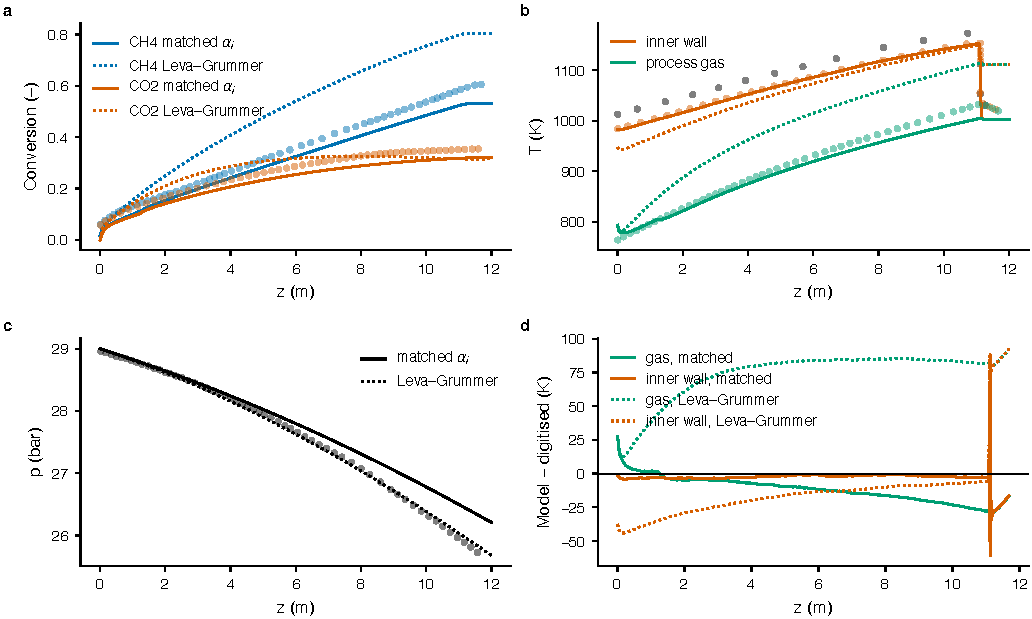
\includegraphics[width=\textwidth]{fig03_validation_xf1989}
\caption{Verification against the digitized industrial case of Xu and Froment~\cite{xu1989b} (symbols) with the digitized outer-wall temperature as boundary condition: (a) methane and CO$_2$ conversion, (b) process-gas and inner-wall temperatures, (c) pressure and (d) temperature residuals, for the matched film coefficient (solid lines) and for the Leva--Grummer correlation with $f_{\mathrm{htg}} = 1$ (dotted).}
\label{fig:xf}
\end{figure}

With the digitized outer-wall temperature prescribed, the response of the tube model is controlled almost entirely by the bed-side film coefficient, and the first finding of the study is that the heat-transfer chain printed in Part~II of Xu and Froment~\cite{xu1989b} does not reproduce their own figure. Evaluated as printed, the De~Wasch--Froment wall coefficient with the Yagi--Kunii dynamic terms gives $\alpha_i \approx 3100$--$3700$~W\,m$^{-2}$\,K$^{-1}$ at the particle Reynolds number of the case ($Re_p \approx 4000$), and the Leva--Grummer correlation gives 940--1580~W\,m$^{-2}$\,K$^{-1}$; the value back-calculated from the digitized wall and gas temperatures and the wall conduction is 348~W\,m$^{-2}$\,K$^{-1}$ (interquartile range 313--363). Used as printed, the correlations overpredict the gas temperature by 70--115~K and the conversion by 0.14--0.22, an RMSE of 75.4~K and 0.160 against 14.0~K and 0.039 for the adopted configuration (Table~S5). Both dynamic terms are linear in $Re\,Pr$ and were established for air an order of magnitude below industrial Reynolds numbers~\cite{dewasch1972,yagi1960}, so the extrapolation drives the effective radial conductivity of the bed to some 50~W\,m$^{-1}$\,K$^{-1}$, which no measurement supports. A displaced decimal in the printed effective-conductivity coefficient (0.014 instead of 0.14) would bring the chain to within 30\,\% of the back-calculated value, but this is a hypothesis rather than a correction.

The Xu--Froment case is therefore used as a verification of the tube model with a matched film coefficient rather than as a validation of the heat-transfer correlation. With $\alpha_i = 348$~W\,m$^{-2}$\,K$^{-1}$ and Latham's inlet effectiveness profile, the model reproduces the digitized profiles with an RMSE of 14.0~K in gas temperature, 16.7~K in inner-wall temperature and 0.015 in the conversion increment along the tube (Fig.~\ref{fig:xf}, Table~S5). The residual offset of about 0.04 in absolute conversion originates in the first half metre and reflects an ambiguity in the digitized inlet that the increment metric removes (Section~S4). This verifies the kinetics, the thermodynamics, the energy balance and the wall-conduction chain. The pressure RMSE rises from 0.04~bar with the Leva--Grummer run to 0.25~bar with the matched coefficient, for the reason given in Section~S5.

\begin{figure}[t]
\centering
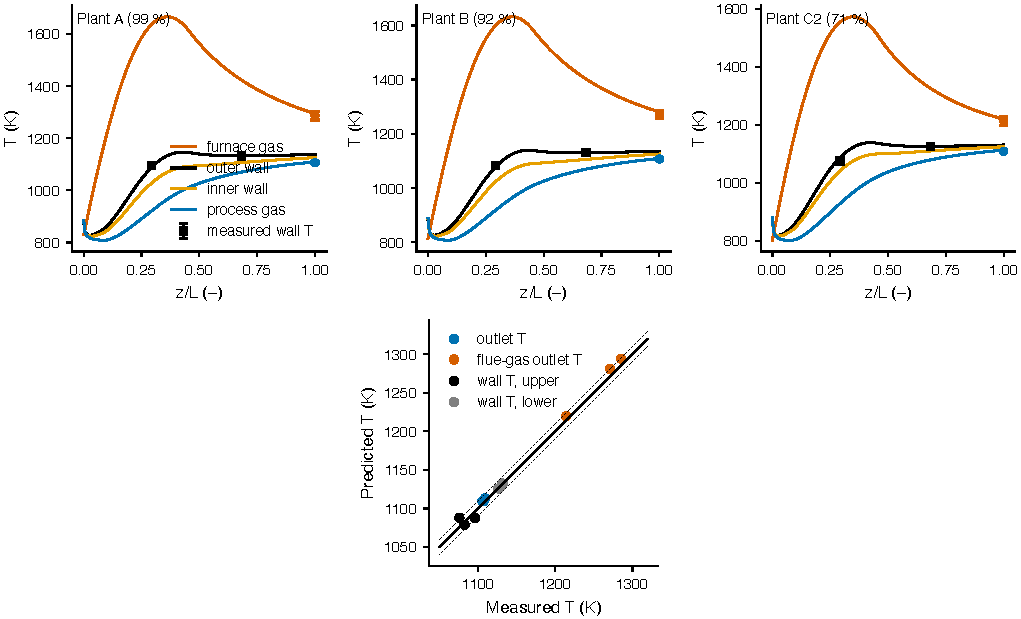
\includegraphics[width=\textwidth]{fig05_latham_calibrated}
\caption{Coupled furnace--tube model after calibration ($\alpha_{\mathrm{top}}$ fixed) on the plant cases of Latham~\cite{latham2008}: axial profiles of furnace-gas, outer-wall, inner-wall and process-gas temperatures for Plants~A, B and C2 with the measured wall temperatures at the two peep-hole elevations, the outlet temperature and the flue-gas outlet temperature (error bars $\pm 1.96\sigma$), and the parity of predicted against measured temperatures (dotted lines $\pm 10$~K).}
\label{fig:latham}
\end{figure}

\begin{table}[t]
\centering\scriptsize
\caption{Plant cases of Latham~\cite{latham2008} (Appendix~H, absolute temperatures) and calibration results: measured inlet and outlet conditions, model errors (predicted minus measured) of the all-cases fit with $\alpha_{\mathrm{top}}$ fixed, and leave-one-case-out held-out errors. Plant~C1 is excluded from the fit (inconsistent feed flow). Per-tube feed; steam-to-carbon ratio on total hydrocarbon carbon; upper and lower wall temperatures at 3.66 and 8.53~m of 12.5~m.}
\label{tab:latham}
\resizebox{\textwidth}{!}{%
\begin{tabular}{lcccccccccccccc}
\toprule
Case & Rate (\%) & $T_{\mathrm{in}}$ (K) & $p_{\mathrm{in}}$ (bar) & Feed (kmol\,h$^{-1}$) & S/C & $T_{\mathrm{out}}$ (K) & $T_{\mathrm{w,u}}$ (K) & $T_{\mathrm{w,l}}$ (K) & $\Delta T_{\mathrm{out}}$ & $\Delta T_{\mathrm{w,u}}$ & $\Delta T_{\mathrm{w,l}}$ & CV $\Delta T_{\mathrm{w,u}}$ & CV $\Delta T_{\mathrm{w,l}}$ \\
\midrule
Plant A  & 99 & 884.5 & 30.06 & 23.5 & 2.89 & 1105.5 & 1095.9 & 1132.0 & $+3.6$ & $-8.4$ & $+0.2$ & $-12.8$ & $+0.7$ \\
Plant B  & 92 & 887.0 & 29.44 & 21.1 & 2.79 & 1107.2 & 1082.3 & 1130.8 & $+2.2$ & $-3.6$ & $-1.1$ & $-5.4$ & $-1.7$ \\
Plant C1 & 96 & 890.9 & 30.27 & 28.7 & 2.85 & 1122.0 & 1111.2 & 1151.5 & -- & -- & -- & -- & -- \\
Plant C2 & 71 & 879.9 & 28.09 & 15.9 & 2.86 & 1108.9 & 1075.7 & 1126.2 & $+3.9$ & $+12.2$ & $-0.5$ & $+18.2$ & $-0.1$ \\
\bottomrule
\end{tabular}}
\end{table}

The bed-side coefficient is validated instead on the plant data, where the furnace model supplies the outer-wall condition and $f_{\mathrm{htg}}$ is a free parameter. Fig.~\ref{fig:latham}, Table~\ref{tab:latham} and Table~S6 summarize the calibration. The adopted fit ($\alpha_{\mathrm{top}}$ fixed) gives $F_{\mathrm{gt}} = 0.323$ [0.309, 0.338], $L_q = 0.456$ [0.434, 0.478] and $f_{\mathrm{htg}} = 1.83$ [1.617, 2.052] as 95\,\% intervals, a $\chi^2$ of 34.9 on 24 degrees of freedom (reduced $\chi^2$ 1.46), and reproduces the outlet temperatures of all three cases within 4~K, the lower wall temperatures within 1.1~K and the upper wall temperatures within 12.2~K. The four-parameter fit lowers $\chi^2$ to 30.5 but is degenerate in $L_q$ and $\alpha_{\mathrm{top}}$ (Table~S6); fixing $\alpha_{\mathrm{top}}$ raises $\chi^2$ by 14\,\%, and the three-parameter fit is adopted for all subsequent work because its parameters are identifiable and its cross-validation folds return nearly the same values ($F_{\mathrm{gt}}$ 0.321--0.326, $L_q$ 0.449--0.465, $f_{\mathrm{htg}}$ 1.79--1.85). The heat-transfer factor of 1.83 is within 9\,\% of the 1.68 obtained by Latham et al.~\cite{latham2011} with a different furnace model on the same plant, and corresponds to a bed-side coefficient of about 1400~W\,m$^{-2}$\,K$^{-1}$ at mid-height of the Plant~A tube, i.e. between the two literature correlations and four times the value that reproduces the Xu--Froment figure; the range 300--3000~W\,m$^{-2}$\,K$^{-1}$ is the epistemic span carried into the uncertainty analysis through $f_{\mathrm{htg}}$.

Leave-one-case-out cross-validation (last two columns of Table~\ref{tab:latham}) shows that the held-out upper-wall temperature is predicted within 5--18~K and the lower within 2~K. The upper-wall error is systematic: Plant~C2, at 71\,\% rate, is predicted too hot at the upper elevation and Plant~A too cold. The upper peep hole lies in the flame zone, where a single parabolic release profile with a load-independent flame length cannot follow the change in flame shape with firing rate. This is the main structural limitation of the furnace model; the residuals are nevertheless within the 15--22~K standard deviation of the wall temperature across the tube population at that elevation~\cite{latham2011}. The consequence for the conclusions is examined in Section~\ref{sec:rq4}.

\begin{figure}[t]
\centering
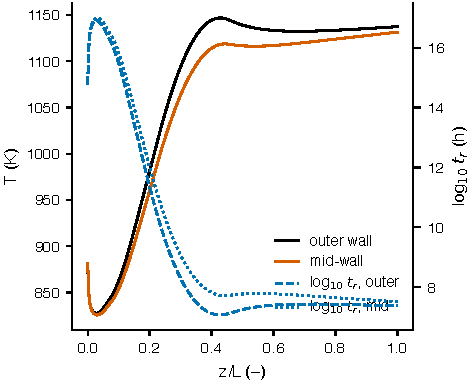
\includegraphics[width=0.7\textwidth]{fig06_creep_life_profile}
\caption{Outer-wall and mid-wall temperature profiles of the calibrated Plant~A tube and the corresponding local rupture time from the Centralloy G 4852 lower scatter band at the local hoop stress; the hot spot governs the life.}
\label{fig:life}
\end{figure}

Fig.~\ref{fig:life} shows the life profile of the calibrated Plant~A tube. The hot spot lies at about 0.43 of the heated length, where the outer wall reaches 1147~K at a hoop stress of 12.9~MPa; the rupture time from the lower scatter band is $10^7$~h at this point, and evaluating the life at the length-averaged outer-wall temperature instead of at the hot spot overstates it by a factor of about 57. The same effect is reported by Yeh~\cite{yeh2021}, there of the order of two hundred; it is smaller here because the master curve of the present alloy is flatter. The absolute value is not credible as a tube life --- the model represents one average tube under creep alone, and the design band of a manufacturer is not the scatter of an installed tube population --- which is why all results below are expressed as ratios.

\subsection{RQ1: what governs hot-spot temperature and life}
\label{sec:rq1}

\begin{figure}[t]
\centering
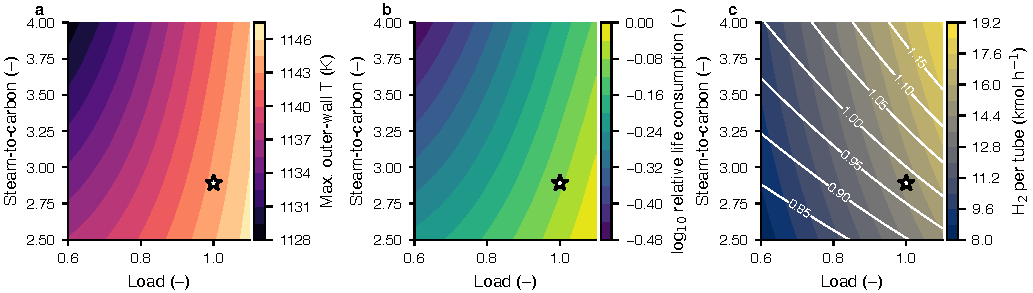
\includegraphics[width=\textwidth]{fig07_operating_maps}
\caption{Closed-loop operating maps in load and steam-to-carbon ratio at constant outlet temperature: (a) hot-spot temperature, (b) $\log_{10}$ of the life consumption relative to the base case and (c) net hydrogen per tube with contours of the firing factor required. The star marks the calibrated Plant~A base.}
\label{fig:maps}
\end{figure}

\begin{figure}[t]
\centering
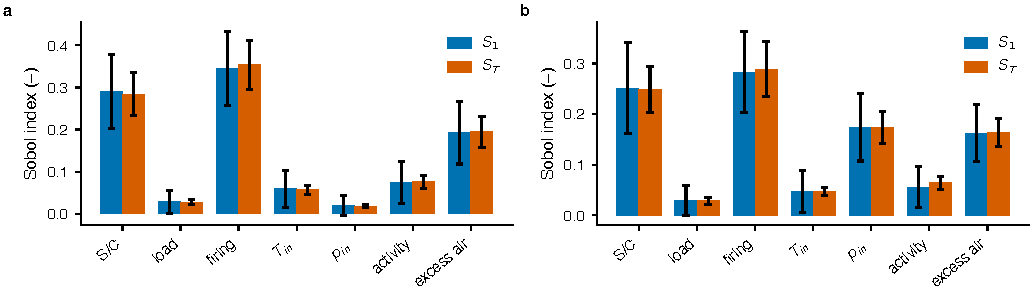
\includegraphics[width=\textwidth]{fig08_sobol}
\caption{First-order ($S_1$) and total-effect ($S_T$) Sobol indices with 95\,\% confidence intervals for (a) the hot-spot temperature and (b) $\log_{10} t_r$ at the hot spot, from the Saltelli design of Table~S8.}
\label{fig:sobol}
\end{figure}

The closed-loop maps (Fig.~\ref{fig:maps}) show the structure of the operating space when the outlet temperature is held by the firing controller. Across the whole grid the hot spot spans only 1128--1146~K. It rises mildly with load: the duty per tube is proportional to the load, and the bed-side coefficient rises almost proportionally with it ($\alpha_i \propto Re^{0.9}$ in the Leva--Grummer correlation), so the film temperature difference is nearly load-independent and only the conduction drop across the wall grows with the flux. It falls with steam-to-carbon ratio because, at the same outlet temperature, the larger process-gas flow raises the bed-side coefficient, the additional steam increases the gas heat capacity, and the equilibrium shift lets the same methane slip be reached with a slightly lower gas temperature, all of which reduce the wall-to-gas temperature difference despite the higher firing needed. The life map (panel~b) is the image of the temperature map through the Larson--Miller relation and spans about half a decade across the space. Hydrogen production (panel~c) increases with both load and steam-to-carbon ratio, the latter through the shift of equilibrium, at the cost of a higher firing factor.

The Sobol analysis over all seven inputs (Fig.~\ref{fig:sobol}, Table~S8) ranks the drivers of the hot-spot temperature as the specific firing factor ($S_T = 0.35$), the steam-to-carbon ratio (0.28) and the excess air (0.19), together 82\,\% of the variance, with the inlet pressure entering $\log_{10} t_r$ at $S_T = 0.17$ through the hoop stress, where it is invisible in the temperature; the remaining indices, the weakness of the interactions and the drivers of the methane slip are given in Section~S7.

The surrogates that make the following campaigns possible are summarized in Fig.~S1 and Table~S4. The Gaussian process is selected for seven of the eight targets, and the physics features improve the hot-spot temperature, outlet temperature and slip. The test RMSE is 0.11~K for the hot-spot temperature and 0.0049 decades for $\log_{10} t_r$, two orders of magnitude below the calibration residuals, at a speed-up of about 4700 relative to the physics model. The position of the hot spot is not learnable ($R^2 = 0.64$) because it is bimodal, an interior maximum near 0.43 of the length for most inputs and an outlet plateau for others; the plateau appears at high firing, where the process gas has caught up with the wall and the local flux at the outlet is small (Section~S11), and it is not needed for the life calculation. The CV+ intervals over-cover: at a nominal level of 0.90 the empirical coverage is 0.94--0.97 for all targets. Over-coverage is expected for CV+, whose guarantee is one-sided, and is conservative; the interval widths are nevertheless small enough (0.25~K for the hot-spot temperature) that surrogate error is immaterial to the conclusions.

\subsection{RQ2: life cost of flexible operation and aging}
\label{sec:rq2}

\begin{figure}[t]
\centering
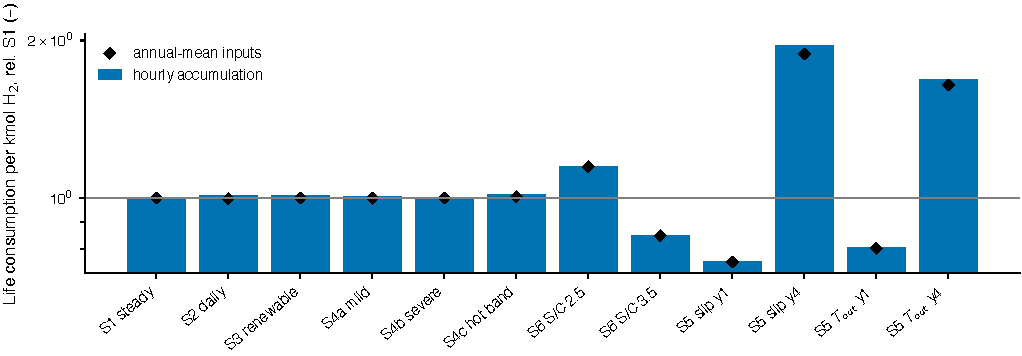
\includegraphics[width=\textwidth]{fig11_scenarios_summary}
\caption{Annual life consumption per kmol of hydrogen relative to the steady base S1 for the RQ2 scenarios, from hourly accumulation (bars) and from a single evaluation at the annual-mean inputs (diamonds).}
\label{fig:scenarios}
\end{figure}

\begin{table}[t]
\centering\scriptsize
\caption{RQ2 scenario summary for one year of the Plant~A twin at the calibrated excess air: hydrogen per tube, Robinson damage $D$, life consumption per kmol~H$_2$ relative to S1, ratio of the annual-mean-condition damage estimate to the hourly-accumulated damage, mean and maximum hot-spot temperature and mean firing factor. Life uses the Centralloy G 4852 lower scatter band ($C = 18.6$).}
\label{tab:scenarios}
\resizebox{\textwidth}{!}{%
\begin{tabular}{lccccccc}
\toprule
Scenario & H$_2$ ($10^3$ kmol) & $D$ (--) & Rel. life cost & Avg.-cond. ratio & $\bar T_{\mathrm{wo,max}}$ (K) & max $T_{\mathrm{wo,max}}$ (K) & Firing \\
\midrule
S1 steady base                    & 128.5 & $6.30\times10^{-4}$ & 1.000 & 1.000 & 1143 & 1143 & 0.978 \\
S2 daily load-following           & 115.7 & $5.72\times10^{-4}$ & 1.010 & 0.987 & 1141 & 1143 & 0.944 \\
S3 renewable-following            & 109.7 & $5.44\times10^{-4}$ & 1.013 & 0.987 & 1140 & 1146 & 0.927 \\
S4a mild over-firing (48 h)       & 128.6 & $6.34\times10^{-4}$ & 1.006 & 0.994 & 1144 & 1157 & 0.979 \\
S4b severe over-firing (6 h)      & 128.5 & $6.32\times10^{-4}$ & 1.003 & 0.997 & 1143 & 1179 & 0.978 \\
S4c hot band $+40$ K (24 h)       & 128.5 & $6.41\times10^{-4}$ & 1.018 & 0.988 & 1144 & 1183 & 0.978 \\
S6 steam-to-carbon 2.5            & 119.9 & $6.74\times10^{-4}$ & 1.147 & 1.000 & 1144 & 1144 & 0.897 \\
S6 steam-to-carbon 3.5            & 139.8 & $5.80\times10^{-4}$ & 0.847 & 1.000 & 1142 & 1142 & 1.092 \\
S5 aging, hold slip, year 1      & 128.5 & $4.77\times10^{-4}$ & 0.756 & 0.998 & 1138 & 1139 & 0.974 \\
S5 aging, hold slip, year 4      & 128.5 & $1.23\times10^{-3}$ & 1.959 & 0.961 & 1156 & 1164 & 0.989 \\
S5 aging, hold $T_{\mathrm{out}}$, year 1 & 129.0 & $5.08\times10^{-4}$ & 0.803 & 0.999 & 1139 & 1140 & 0.982 \\
S5 aging, hold $T_{\mathrm{out}}$, year 4 & 127.4 & $1.05\times10^{-3}$ & 1.686 & 0.975 & 1153 & 1159 & 0.969 \\
\bottomrule
\end{tabular}}
\end{table}

Table~\ref{tab:scenarios} and Fig.~\ref{fig:scenarios} answer RQ2 for one year of operation at the calibrated base. Under the outlet-temperature controller, load-following is life-neutral: the daily profile (S2) and the renewable-following profile (S3) consume 1.010 and 1.013 of the S1 life per kmol~H$_2$. Two effects nearly cancel. The hot-spot temperature falls with load at constant outlet temperature (Fig.~\ref{fig:maps}a), so the hours at reduced load save life, while the hours at overload cost it; which one wins is decided by the local slope of the master curve, and the margin is smaller than the uncertainty on that slope. The statement that S2 costs no more than S1 holds in 0.43 of the Monte Carlo samples (Table~\ref{tab:robust}) and its sign changes with the alloy (Section~\ref{sec:rq4}), so the defensible statement is that smooth load variation changes the life cost per kmol by less than 2\,\% in either direction and that the sign is not resolved. Hydrogen output falls by 10\,\% and 15\,\% respectively, so the absolute annual damage falls in proportion. A steady-state assessment at the annual-mean inputs reproduces the hourly accumulation within 2\,\% for every scenario without discrete events (ratio 0.987 for S3), which means that the non-linearity of the Larson--Miller relation is not strong enough over this load range to make time-resolved simulation necessary for smooth load changes. The conclusion is conditional on the controller: without outlet-temperature (or slip) control, a load reduction at unchanged firing raises the hot spot sharply, and the open-loop design shows life-consumption ratios of up to 40 times the base when high firing coincides with a hot inlet; the operating discipline of controlling on the outlet is itself the main protection of the tubes.

Discrete over-firing events are different in kind. During a mild event ($+10$\,\% firing) the damage rate is 2.1~times the base rate, during a severe event ($+25$\,\%) it is 4.9~times, and a 40~K hot band raises it by a factor of 7.4; but because the events are short, their share of the annual damage is 0.3--1.7\,\% and the annual life cost per kmol rises by at most 2\,\%. The annual-mean evaluation underestimates the event scenarios (diamonds below bars in Fig.~\ref{fig:scenarios}), as it must for a convex damage law, but the error is small at these event frequencies. The steam-to-carbon ratio has a larger steady effect: operating at 2.5 costs 1.15 and at 3.5 costs 0.85 of the S1 life per kmol~H$_2$, because the higher ratio both cools the hot spot and raises the hydrogen yield.

Catalyst aging dominates every operational effect. With the activity falling from 0.30 to 0.10 over four years, a range that brackets the mid-campaign value of 0.20 fitted to the plant and is consistent with the rapid initial deactivation followed by a slow decline observed for fresh catalyst~\cite{xu1989a} and with the four-year catalyst life of the reference plant~\cite{latham2011}, and with the controller holding the methane slip, the life cost per kmol~H$_2$ rises from 0.76 in the first year (fresh catalyst) to 1.96 in the fourth as the hot spot climbs from 1138 to 1164~K; holding the outlet temperature instead gives 1.69 in the fourth year because the slip is allowed to rise. Over the campaign the life consumed in year~4 is two and a half times that in year~1, and the question of when to change the catalyst is therefore also a tube-life question. The ranking here is by creep-life cost alone. Rainflow counting of the hourly wall-gradient histories (Section~S11) shows a year of daily load-following matching one start-up and shutdown only for a fatigue exponent below about 4.2, against the two to six cool-downs a plant undergoes each year; thermal cycling does not overturn the ranking, although creep--fatigue interaction remains outside the model.

\subsection{RQ3: Pareto-optimal regimes and the steam credit}
\label{sec:rq3}

\begin{figure}[t]
\centering
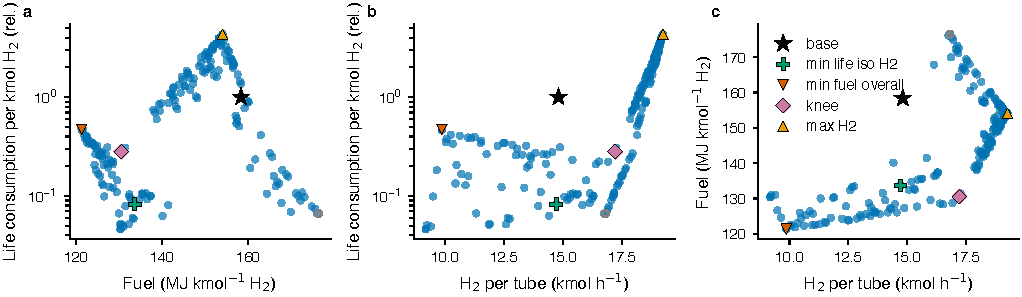
\includegraphics[width=\textwidth]{fig12_pareto}
\caption{Physics-verified NSGA-II Pareto set in (a) firebox fuel per kmol~H$_2$ against life consumption per kmol~H$_2$, (b) net hydrogen per tube against life consumption and (c) hydrogen against fuel; open circles are members infeasible under the physics model, and the marked regimes are listed in Table~\ref{tab:regimes}.}
\label{fig:pareto}
\end{figure}

\begin{table}[t]
\centering\scriptsize
\caption{RQ3 representative regimes, physics-verified, from the NSGA-II Pareto set. Fuel is firebox fuel per kmol~H$_2$; life is the consumption rate per kmol~H$_2$ relative to the base (G 4852 lower scatter band).}
\label{tab:regimes}
\resizebox{\textwidth}{!}{%
\begin{tabular}{lcccccccccc}
\toprule
Regime & Load & S/C & $T_{\mathrm{in}}$ (K) & Excess air (\%) & Firing & H$_2$ (kmol\,h$^{-1}$) & Fuel (MJ\,kmol$^{-1}$) & Rel. life cost & $T_{\mathrm{wo,max}}$ (K) & CH$_4$ slip (\%) \\
\midrule
base              & 1.00 & 2.89 & 885 & 21.6 & 1.000 & 14.82 & 158.4 & 1.000 & 1147 & 7.81 \\
min life, iso-H$_2$ & 0.97 & 4.00 & 897 & 17.6 & 0.872 & 14.87 & 133.7 & 0.123 & 1108 & 7.80 \\
knee              & 1.10 & 4.00 & 893 & 5.4 & 0.866 & 17.06 & 131.0 & 0.281 & 1127 & 7.42 \\
max H$_2$         & 1.10 & 4.00 & 900 & 5.0 & 1.150 & 19.26 & 154.1 & 3.220 & 1177 & 3.89 \\
min fuel overall  & 0.60 & 4.00 & 900 & 5.0 & 0.850 & 9.87 & 121.3 & 0.575 & 1128 & 5.72 \\
min life overall  & 0.62 & 4.00 & 823 & 24.5 & 0.897 & 9.56 & 137.5 & 0.084 & 1092 & 7.80 \\
\bottomrule
\end{tabular}}
\end{table}

The Pareto set (Fig.~\ref{fig:pareto}, Table~\ref{tab:regimes}) contains 200 members, of which 198 remain feasible under the physics model; the maximum discrepancy between surrogate and physics on the set is 0.03 in relative life and below 0.1~MJ\,kmol$^{-1}$ in fuel. The calibrated base is dominated by 37 members. The knee of the front raises hydrogen by $+15$\,\% while cutting fuel per kmol by $-17$\,\% and life consumption per kmol to 0.28 of the base; it does so by running at 110\,\% load with the minimum excess air, a high inlet temperature and a lower firing factor. At constant production the life cost falls to 0.12 of the base, an eightfold reduction obtained purely by reducing the firing and letting the hot spot fall from 1147 to 1108\,K, at $-16$\,\% fuel. The maximum-hydrogen corner ($+30$\,\%) costs 3.2~times the base life per kmol and runs close to the wall-temperature limit.

\begin{figure}[t]
\centering
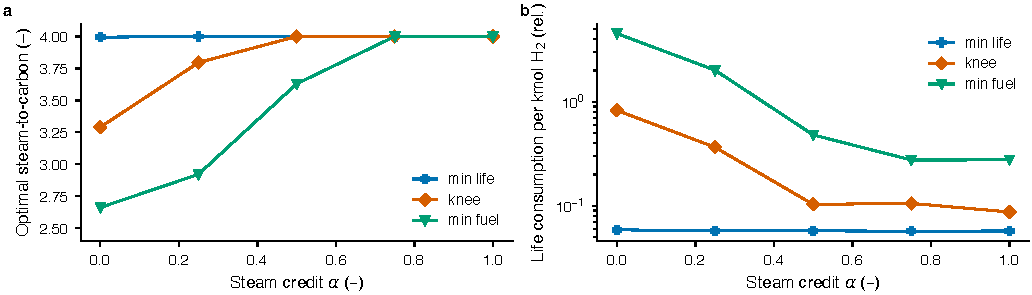
\includegraphics[width=\textwidth]{fig13_steam_credit}
\caption{Iso-production front as a function of the steam credit $\alpha$: (a) optimal steam-to-carbon ratio and (b) life consumption per kmol~H$_2$ relative to the base for the minimum-life, knee and minimum-fuel regimes. The full sweep is given in Table~S7.}
\label{fig:steam}
\end{figure}

Every member of the front sits at the upper bound of the steam-to-carbon ratio (3.96--4.00). This is an artefact of the objective: with firebox fuel alone, additional steam is free, and the equilibrium shift and the cooling of the hot spot both favor maximum steam. The steam-credit sweep (Fig.~\ref{fig:steam}, Table~S7) shows how the answer changes when steam raising and feed preheat are charged. With steam fully charged ($\alpha = 0$) the minimum-fuel regime moves to a steam-to-carbon ratio of 2.64 and the knee to 3.4, while the minimum-life regime stays at 4.0 but now costs $+4.1$\,\% more total fuel than the base for a life cost of 0.094. For $\alpha \geq 0.75$ the ratio of 4.0 is optimal for all three regimes, and already at $\alpha = 0.5$ the minimum-fuel regime sits at 3.7, close to the bound. In a hydrogen plant the process steam is raised in the waste-heat boiler on the reformer effluent and in the flue-gas convection section, and the surplus is exported, so the marginal steam for a higher ratio mostly displaces export steam rather than requiring extra fuel; this corresponds to $\alpha$ between about 0.5 and 1 depending on the value the site attaches to export steam, and places most plants in the region where tube life and fuel economy pull in the same direction. The plant's own steam balance, not the reformer, therefore decides whether running steam-rich is a life-saving measure or a fuel penalty, and the twin makes the dependence explicit.

\subsection{RQ4: uncertainty and robustness}
\label{sec:rq4}

\begin{figure}[t]
\centering
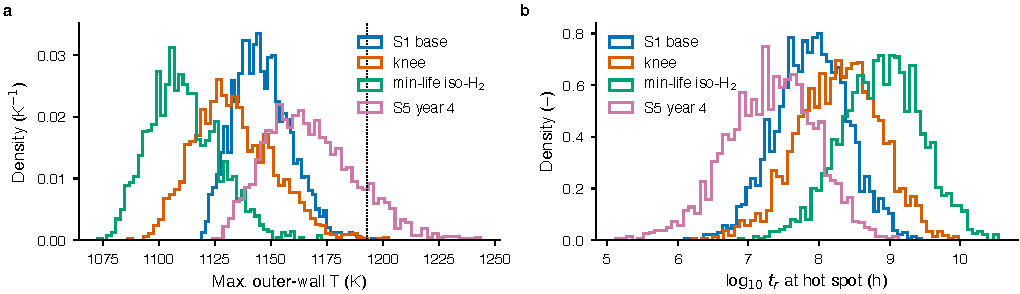
\includegraphics[width=\textwidth]{fig14_uq_distributions}
\caption{Monte Carlo distributions of all uncertainty groups through the physics model: (a) the hot-spot temperature, with the design limit, and (b) $\log_{10} t_r$ at the hot spot, at the S1 base, the RQ3 knee, the iso-H$_2$ minimum-life regime and the end of the fourth aging year.}
\label{fig:uq}
\end{figure}

\begin{table}[t]
\centering\footnotesize
\caption{RQ4 Monte Carlo (scrambled Sobol design, all uncertainty groups) through the physics model: median and 5--95\,\% interval of the hot-spot temperature, of $\log_{10} t_r$ and of the paired life consumption per kmol~H$_2$ relative to the base.}
\label{tab:uq}
\begin{tabular}{lccc}
\toprule
Operating point & $T_{\mathrm{wo,max}}$ (K) & $\log_{10} t_r$ (h) & Rel. life cost \\
\midrule
S1 base                  & 1145 [1127, 1169] & 7.06 [5.94, 8.20] & 1.000 (paired) \\
RQ3 knee                 & 1128 [1103, 1161] & 7.47 [6.26, 8.63] & 0.329 [0.213, 0.561] \\
RQ3 min-life, iso-H$_2$  & 1110 [1088, 1138] & 7.90 [6.69, 9.06] & 0.143 [0.107, 0.212] \\
S5 year 4, hold slip     & 1165 [1138, 1203] & 6.60 [5.34, 7.79] & 2.823 [1.657, 6.242] \\
S/C 2.5                  & 1146 [1129, 1166] & 7.03 [5.93, 8.18] & 1.140 [0.941, 1.315] \\
S/C 3.5                  & 1144 [1127, 1172] & 7.11 [5.94, 8.25] & 0.857 [0.623, 1.083] \\
load 0.70                & 1138 [1123, 1156] & 7.20 [6.09, 8.34] & 1.034 [0.732, 1.384] \\
load 0.85                & 1141 [1124, 1162] & 7.13 [6.02, 8.28] & 0.989 [0.841, 1.170] \\
\bottomrule
\end{tabular}
\end{table}

\begin{table}[t]
\centering\footnotesize
\caption{Robustness of the RQ2/RQ3 conclusions: fraction of paired Monte Carlo samples
supporting each statement, as a function of the exponent $p$ in a structural variant where
the flame length shrinks with load as $L_q\,\mathrm{load}^{p}$. The calibrated model is
$p = 0$; $p = 0.5$ is the bound discussed in Section~\ref{sec:flame}. The first and third
rows involve only full-load operating points, where $\mathrm{load}^{p} = 1$, so they cannot
move with $p$ and serve as a check on the sampling.}
\label{tab:robust}
\begin{tabular}{lcccccc}
\toprule
Statement & $p = 0$ & 0.1 & 0.2 & 0.25 & 0.5 & 1.0 \\
\midrule
aging year 4 costs $> 2\times$ S1 life per kmol & 0.819 & 0.819 & 0.819 & 0.819 & 0.819 & 0.819 \\
knee regime $< 0.5\times$ base                  & 0.885 & 0.911 & 0.928 & 0.936 & 0.974 & 0.997 \\
S/C 3.5 cheaper in life than S/C 2.5            & 0.856 & 0.856 & 0.856 & 0.856 & 0.856 & 0.856 \\
S2 daily $\leq$ S1                              & 0.425 & 0.265 & 0.116 & 0.067 & 0.000 & 0.000 \\
S3 renewable $\leq$ S1                          & 0.484 & 0.320 & 0.168 & 0.105 & 0.000 & 0.000 \\
\bottomrule
\end{tabular}
\end{table}

Table~\ref{tab:uq} and Fig.~\ref{fig:uq} give the propagated uncertainty. At the base point the 90\,\% interval of the hot-spot temperature is 42~K wide and that of $\log_{10} t_r$ spans 5.94--8.20, i.e. a factor of about 180 in absolute rupture time. The paired ratios are much tighter: the knee regime costs 0.21--0.56 of the base life per kmol and the fourth aging year 1.7--6.2 times, so the ranking of regimes survives an uncertainty that makes the absolute life meaningless. The nominal result lies inside the 90\,\% interval at every point, and the end-of-campaign hot spot exceeds the 1193\,K limit in about 8\,\% of the samples.

The variance decomposition (Fig.~S2, Table~S9) attributes 86\,\% of the variance of $\log_{10} t_r$ to the creep group, dominated by the scatter of the rupture band and the Larson--Miller constant, 9\,\% to the kinetics, 3\,\% to the wall-temperature measurement and 2\,\% to the calibrated heat-transfer parameters. For the hot-spot temperature the kinetics group dominates (51\,\%), followed by the measurement offset and the wall thickness; that decomposition is identical to every printed digit on all four rupture curves tested, because the alloy enters the thermal problem only through the wall thickness and the tube conductivity. The one-at-a-time shares sum to within 0.04 of one and the Sobol total effects on the surrogate confirm the ranking, so the groups act almost additively.

The robustness fractions (Table~\ref{tab:robust}) state which conclusions hold across the joint uncertainty. That the knee regime halves the life cost holds in 0.89 of the samples, that steam-to-carbon 3.5 is cheaper in life than 2.5 in 0.86, and that the fourth aging year costs more than twice the S1 life per kmol in 0.82; repeating the analysis on the other three curves leaves all three between 0.82 and 0.94, so they are properties of the process rather than of the alloy. The flexibility statements are different in kind. At the calibrated flame length they already hold in fewer than half of the samples, 0.43 and 0.48, and Table~\ref{tab:robust} shows how quickly that support goes: an exponent of 0.1, barely distinguishable from a constant flame length, cuts both by a third; by 0.3 they are 0.03 and 0.06, and at 0.5 neither survives. The material conclusions are untouched across the range --- the knee strengthens from 0.885 to 0.997 --- and hold on all four rupture curves, while the flexibility fractions cross 0.5 with the curve too (0.55 and 0.62 on the two with the higher Larson--Miller constant). The flame-length response to load (Section~\ref{sec:flame}) and the local slope of the master curve, neither identifiable from the published data, decide the sign of an effect whose magnitude is under 2\,\%.

All of the above describes one average tube. Because damage is convex in wall temperature, spreading a per-tube offset over the 336 tubes of the reference furnace (Section~S10) raises the population-mean damage rate above the average tube's by 1.29 to 1.75 for a population standard deviation of 15 to 22~K; the hottest decile consumes life 3.9 to 7.4 times faster and the hottest tube by an order of magnitude. The correction varies little between regimes, leaving the ranking by life per kmol~H$_2$ unchanged.

% =====================================================================
\section{Discussion}
\label{sec:discussion}

\subsection{Industrial implications}

Three results have direct operational consequences. First, of the three drivers identified in Section~\ref{sec:rq1}, excess air is the least appreciated: at fixed fuel it lowers the hot-spot temperature by shifting heat release down the tube. Its efficiency penalty, the larger flue-gas flow and stack loss, enters through the firing required to hold the outlet temperature, so the optimizer weighs it against life rather than ignoring it. Excess air is also the cheapest variable to move on an operating plant, and its effect can be verified with the existing pyrometer survey.

Second, whether the gains of the knee regime are realizable depends on constraints outside the twin: preheat-coil metallurgy at 900~K inlet temperature, pressure-swing-adsorption capacity at 110\,\% load and the downstream steam balance. The steam-credit sweep shows the recommended steam-to-carbon ratio moving from 4.0 to about 2.7 depending on how the plant values steam; the twin cannot decide this, but it makes the dependence explicit.

Third, provided the outlet temperature is controlled, a plant that must follow demand should not fear the tube-life consequences of smooth load changes in either direction, but should watch the end-of-campaign hot-spot temperature under a methane-slip target. That the load-following conclusions are the least robust of the study reflects the size of the nominal effect (a factor of 2.0 against 1\,\%), not a difference in modeling quality, and we recommend that digital-twin studies report robustness fractions alongside nominal results so that small nominal effects are not mistaken for findings.

\subsection{The flame-length response to load as a measurement need}
\label{sec:flame}

The one structural assumption that changes a conclusion is how the heat-release profile of the burners responds to the firing rate. The calibrated model uses a single dimensionless flame length, and the cross-validation residuals at the upper peep hole (Section~\ref{sec:verification}) already show that this is the weakest element of the model: the partially loaded Plant~C2 is predicted too hot at the top and the fully loaded Plant~A too cold. When the flame is allowed to shorten with load, the flexible-operation conclusion reverses because the hot spot at reduced load moves into a hotter part of the furnace. The two hypotheses correspond to two ways of turning a furnace down: reducing the fuel flow through all burners, which leaves the length of a turbulent diffusion flame nearly unchanged~\cite{hawthorne1949}, or taking burner rows out of service, which redistributes the heat release; the three published operating points cannot separate them. What would settle the question is a pyrometer survey at three or four elevations at two or three firing rates on one furnace, which most plants already perform in part during turnaround planning; a digital twin of the kind presented here turns such a survey into an estimate of the flame-length response with its uncertainty. The requirement is demanding: the sweep of Table~\ref{tab:robust} shows that an exponent of 0.1 already changes the answer materially, and the wall-temperature signature of that difference is about 9~K at the upper peep hole at 70\,\% load and below 0.1~K at the lower, in both cases smaller than the 15--22~K spread of the tube population, so a single elevation at a single firing rate cannot resolve it however accurate the instrument. Such a survey would not rescue the flexibility conclusions --- at the calibrated flame length they already sit below even odds --- but it would replace an unresolved sign with a quantified one, and it would do so for the two statements that the present data cannot decide. We regard this as the single most valuable measurement for tube-life-aware operation of top-fired reformers.

\subsection{Limitations}

The model represents one average tube. Tube-to-tube variation in a top-fired furnace, caused by burner imbalance, row position and flow maldistribution, has a standard deviation of 15--22~K across the tube population at a given elevation in the reference furnace~\cite{latham2011}. Section~S10 propagates that scatter through the rupture curve: the population mean exceeds the average tube by about 1.5 in damage rate, the hottest decile by 5.3 and the hottest of 336 tubes --- the one that decides when the furnace is retubed --- by 16.5 at $\sigma = 18.5$~K. Two things bound the last figure: the scatter is assumed normal and the hottest tube is the extreme of that assumed tail, so the hottest decile is the more robust statistic; and the maximum of a bundle is itself a random variable, with a 5--95\,\% range of 8.3--25.3 over repeated bundles. The measurement group of the uncertainty analysis ($\pm 10$~K) is a different quantity, an epistemic offset of the pyrometer reference common to all tubes rather than the spread between them, and the two are not combined. A per-tube wall-temperature distribution measured by a pyrometer survey would replace the assumed normal and would also bound the tail directly.

The life model covers creep only. Thermal fatigue during start-up and shutdown, creep--fatigue interaction and carburisation are not modeled, and the hoop stress is the pressure stress alone. The elastic thermal stress from the radial temperature gradient is 110~MPa at the hot spot, close to an order of magnitude above the 12.9~MPa hoop stress, and 63~MPa averaged over the heated length (Section~S1); in steady operation it relaxes by creep and is conventionally excluded from the design stress, but it is the driver of damage during thermal cycling. The scenario results should therefore be read as the creep-life cost of the scenarios, not their total life cost. The cyclic content of each scenario is screened in Section~S11: smooth load variation adds a fatigue exposure small compared with the start-up and shutdown cycles a plant already accepts, so the ranking of the flexible-operation scenarios is unlikely to change if thermal cycles were counted, but creep--fatigue interaction and carburisation remain outside the model.

The rupture curve is a manufacturer design band, not a heat-resolved data set. The Average and Lower Scatter Band curves of the G 4852 sheet describe the manufacturer's own qualification population at a 95\,\% confidence level; they are not the heat-to-heat spread of the tubes installed in a particular furnace, and the alloy of the reference plant is not stated. Absolute rupture times therefore remain implausible as tube lives ($10^7$~h at the calibrated hot spot), and all results are reported as ratios; the ratios themselves keep their direction on all four curves tested. Rupture data resolved by heat, from the NIMS data sheets or from rupture points tabulated in the open literature~\cite{whittaker2013,haidemenopoulos2021}, would replace the design band by a measured scatter distribution and is the remaining step towards any absolute statement.

The scenarios are quasi-steady: each hour is a steady state of the twin, and the thermal inertia of the tube, the catalyst and the furnace refractory is neglected. The tube follows hourly load changes essentially instantaneously while the refractory lags them (Section~S1); for load ramps of 0.1 per hour and events of one hour or longer the quasi-steady approximation is reasonable for the tube, but it excludes the transient overshoot of the wall temperature during a fast firing step, which would increase the cost of the over-firing events. Finally, the calibration rests on three operating points of one furnace, so the parameter intervals are conditional on that furnace and transfer to another reformer requires recalibration on its own survey data.

% =====================================================================
\section{Conclusions}
\label{sec:conclusions}

A physics-informed digital twin of an industrial top-fired steam methane reformer has been built from published kinetics, plant data and creep curves, coupling a one-dimensional tube model, a long-furnace model, a Larson--Miller life module, Gaussian-process surrogates with conformal prediction intervals and Monte Carlo uncertainty propagation in one open, versioned pipeline.
\begin{itemize}
\item The tube model reproduces the industrial case of Xu and Froment within 14~K in gas temperature once the film coefficient is matched, and the heat-transfer correlations printed in that paper are found to overpredict the film coefficient by an order of magnitude at industrial Reynolds numbers. The coupled model calibrated on three plant operating points reproduces outlet temperatures within 4~K and wall temperatures within 12~K, with identifiable parameters and a systematic residual at the upper elevation that points to the flame-length response to load.
\item Firing intensity, steam-to-carbon ratio and excess air explain 82\,\% of the variance of the hot-spot temperature with negligible interactions; inlet pressure enters the life only through the hoop stress.
\item Under outlet-temperature control, load-following and renewable-following change the life cost per kmol of hydrogen by less than 2\,\%, short over-firing events by at most 2\,\%, and the steam-to-carbon ratio by $\pm 15$\,\%; catalyst aging under a methane-slip target doubles the life cost in four years; the cyclic thermal exposure of smooth load variation is small against the plant's own start-up cycles.
\item The calibrated base is Pareto-dominated: a knee regime gives $+15$\,\% hydrogen at $-17$\,\% fuel per kmol and 0.28 of the life cost, and at constant production the life cost can be cut to 0.12. The optimal steam-to-carbon ratio depends on the steam credit, moving from 4.0 to 2.7 when steam raising is charged in full.
\item The 90\,\% uncertainty on the absolute rupture time spans a factor of about 180, dominated by creep-curve scatter (86\,\%), while paired ratios between regimes remain tight. The aging, knee and steam-to-carbon conclusions hold in 82\,\% to 88\,\% of the samples on the base curve and in 82\,\% to 94\,\% across four rupture curves; the flexible-operation conclusion is supported in fewer than half the samples even at the calibrated flame length, and disappears entirely under any appreciable load dependence of the flame length or a change of rupture curve.
\end{itemize}
The next steps are rupture data resolved by heat for the HP-Nb and HK40 families, a measured per-tube wall-temperature distribution to replace the normal scatter assumed in the population extension, and, above all, a multi-elevation pyrometer survey at several firing rates. The sign of the life cost of flexible operation is decided jointly by the flame-length response to load and by the local slope of the rupture curve, and neither is identified by the published data.

% =====================================================================
\section*{Data and code availability}
The model code (\texttt{rdt} package), the pipeline entry point (\texttt{python -m rdt.pipeline --stage all --version v3}), the transcribed literature data with their provenance annotations, the digitized verification curves, all v3 result files and the scripts that generate every figure, table and number in this manuscript are available at \url{https://github.com/IzbassarO/reformer-digital-twin} and archived at \todo{Zenodo DOI}. The literature PDFs are not redistributed. Transcribed data are released under CC~BY~4.0 and code under the MIT license.

\section*{CRediT authorship contribution statement}
\textbf{Madina Sissenbay:} Conceptualization, Methodology, Validation, Investigation, Resources, Supervision, Project administration, Writing -- review \& editing.
\textbf{Izbassar Orynbassar:} Conceptualization, Methodology, Software, Formal analysis, Data curation, Visualization, Writing -- original draft, Writing -- review \& editing.

\section*{Declaration of generative AI and AI-assisted technologies in the writing process}
During the preparation of this work the authors used Claude (Anthropic) in order to assist with code development, data transcription checks, figure and table generation and drafting of the text. After using this tool, the authors reviewed and edited the content as needed and take full responsibility for the content of the published article.

\section*{Declaration of competing interest}
The authors declare that they have no known competing financial interests or personal relationships that could have appeared to influence the work reported in this paper. M.S. is employed in the industrial gas sector; the work uses exclusively published data and no proprietary information from any employer.

\section*{Funding}
This research did not receive any specific grant from funding agencies in the public, commercial, or not-for-profit sectors.

\section*{Acknowledgements}
I.O. acknowledges the support of the Bolashak International Scholarship of the Republic of Kazakhstan during the preparation of this work. The authors thank D.~A. Latham for the publicly archived thesis appendix that made the plant-scale calibration possible.

% =====================================================================
\begin{thebibliography}{99}
\setlength{\itemsep}{0pt}

\bibitem{iea2024} International Energy Agency, Global Hydrogen Review 2024, IEA, Paris, 2024.

\bibitem{latham2011} D.~A. Latham, K.~B. McAuley, B.~A. Peppley, T.~M. Raybold, Mathematical modeling of an industrial steam-methane reformer for on-line deployment, Fuel Process. Technol. 92 (2011) 1574--1586. \url{https://doi.org/10.1016/j.fuproc.2011.04.001}

\bibitem{ray2003} A.~K. Ray, S.~K. Sinha, Y.~N. Tiwari, J. Swaminathan, G. Das, S. Chaudhuri, R. Singh, Analysis of failed reformer tubes, Eng. Fail. Anal. 10 (2003) 351--362. \url{https://doi.org/10.1016/S1350-6307(02)00029-8}

\bibitem{api530} American Petroleum Institute, API Standard 530: Calculation of Heater-Tube Thickness in Petroleum Refineries, 7th ed., API, Washington, DC, 2015.

\bibitem{xu1989a} J. Xu, G.~F. Froment, Methane steam reforming, methanation and water-gas shift: I. Intrinsic kinetics, AIChE J. 35 (1989) 88--96. \url{https://doi.org/10.1002/aic.690350109}

\bibitem{xu1989b} J. Xu, G.~F. Froment, Methane steam reforming: II. Diffusional limitations and reactor simulation, AIChE J. 35 (1989) 97--103. \url{https://doi.org/10.1002/aic.690350110}

\bibitem{pantoleontos2012} G. Pantoleontos, E.~S. Kikkinides, M.~C. Georgiadis, A heterogeneous dynamic model for the simulation and optimisation of the steam methane reforming reactor, Int. J. Hydrogen Energy 37 (2012) 16346--16358. \url{https://doi.org/10.1016/j.ijhydene.2012.02.125}

\bibitem{plehiers1989} P.~M. Plehiers, G.~F. Froment, Coupled simulation of heat transfer and reaction in a steam reforming furnace, Chem. Eng. Technol. 12 (1989) 20--26. \url{https://doi.org/10.1002/ceat.270120105}

\bibitem{zamaniyan2008} A. Zamaniyan, H. Ebrahimi, J.~S.~S. Mohammadzadeh, A unified model for top fired methane steam reformers using three-dimensional zonal analysis, Chem. Eng. Process. 47 (2008) 946--956. \url{https://doi.org/10.1016/j.cep.2007.03.005}

\bibitem{kumar2015} A. Kumar, M. Baldea, T.~F. Edgar, O.~A. Ezekoye, Smart manufacturing approach for efficient operation of industrial steam-methane reformers, Ind. Eng. Chem. Res. 54 (2015) 4360--4370. \url{https://doi.org/10.1021/ie504087z}

\bibitem{jafarizadeh2024} A. Jafarizadeh, M. Panjepour, M.~D. Emami, Advanced modelling and optimization of steam methane reforming: from CFD simulation to machine learning-driven optimization, Int. J. Hydrogen Energy 96 (2024) 1262--1280. \url{https://doi.org/10.1016/j.ijhydene.2024.11.352}

\bibitem{yerimah2025} L.~E. Yerimah, M. Mehana, R.~P. Singh, P. Sharan, Uncertainty-aware hydrogen production optimization from a steam methane reformer with a water gas shift reactor and pressure swing adsorption, Ind. Eng. Chem. Res. 64 (2025) 18298--18314. \url{https://doi.org/10.1021/acs.iecr.5c01681}

\bibitem{nabavi2025} S.~R. Nabavi, Z. Guo, Z. Wang, Machine learning-assisted surrogate modeling with multi-objective optimization and decision-making of a steam methane reforming reactor, arXiv:2507.07641 (2025). \url{https://arxiv.org/abs/2507.07641}

\bibitem{nims16b} National Institute for Materials Science, Data sheets on the elevated-temperature properties of centrifugally cast 25Cr-20Ni-0.4C steel tubes for use in reformer furnaces (SCH 22-CF), NIMS Creep Data Sheet No. 16B, Tsukuba, Japan. \url{https://doi.org/10.11503/nims.1020}

\bibitem{nims38a} National Institute for Materials Science, Data sheets on the elevated-temperature properties of centrifugally cast tubes and cast block of 25Cr-35Ni-0.4C steel for reformer furnaces (SCH 24), NIMS Creep Data Sheet No. 38A, Tsukuba, Japan. \url{https://doi.org/10.11503/nims.1042}

\bibitem{matnavi_terms} National Institute for Materials Science, MatNavi Service Terms of Use, NIMS, Tsukuba, Japan. \url{https://mits.nims.go.jp/agreement/MatNavi_agreement_en.pdf}

\bibitem{latham2008} D.~A. Latham, Mathematical modelling of an industrial steam methane reformer, M.Sc.E. thesis, Department of Chemical Engineering, Queen's University, Kingston, Ontario, Canada, 2008. \url{http://hdl.handle.net/1974/1650}

\bibitem{lao2016} L. Lao, A. Aguirre, A. Tran, Z. Wu, H. Durand, P.~D. Christofides, CFD modeling and control of a steam methane reforming reactor, Chem. Eng. Sci. 148 (2016) 78--92. \url{https://doi.org/10.1016/j.ces.2016.03.038}

\bibitem{tran2017} A. Tran, A. Aguirre, M. Crose, H. Durand, P.~D. Christofides, Temperature balancing in steam methane reforming furnace via an integrated CFD/data-based optimization approach, Comput. Chem. Eng. 104 (2017) 185--200. \url{https://doi.org/10.1016/j.compchemeng.2017.04.013}

\bibitem{kumar2017} A. Kumar, M. Baldea, T.~F. Edgar, A physics-based model for industrial steam-methane reformer optimization with non-uniform temperature field, Comput. Chem. Eng. 105 (2017) 224--236. \url{https://doi.org/10.1016/j.compchemeng.2017.01.002}

\bibitem{whittaker2013} M. Whittaker, B. Wilshire, J. Brear, Creep fracture of the centrifugally-cast superaustenitic steels, HK40 and HP40, Mater. Sci. Eng. A 580 (2013) 391--396. \url{https://doi.org/10.1016/j.msea.2013.05.041}

\bibitem{haidemenopoulos2021} G.~N. Haidemenopoulos, A.~D. Zervaki, H. Kamoutsi, K. Polychronopoulou, Creep rupture in HP-Nb refractory steel tubes due to short-term overheating, Eur. J. Mater. 1 (2021) 1--22. \url{https://doi.org/10.1080/26889277.2021.1994841}

\bibitem{guguloth2023} K. Guguloth, N. Roy, Creep life estimation of reformer alloy using $\theta$-projection method -- a neuro fuzzy approach, Int. J. Press. Vessels Piping 203 (2023) 104938. \url{https://doi.org/10.1016/j.ijpvp.2023.104938}

\bibitem{yeh2021} C.-L. Yeh, Effect of burner operation on the catalyst tube lifetime of a steam methane reformer: a numerical study, Appl. Sci. 11 (2021) 231. \url{https://doi.org/10.3390/app11010231}

\bibitem{larson1952} F.~R. Larson, J. Miller, A time-temperature relationship for rupture and creep stresses, Trans. ASME 74 (1952) 765--775.

\bibitem{robinson1952} E.~L. Robinson, Effect of temperature variation on the long-time rupture strength of steels, Trans. ASME 74 (1952) 777--781.

\bibitem{cantera} D.~G. Goodwin, H.~K. Moffat, I. Schoegl, R.~L. Speth, B.~W. Weber, Cantera: an object-oriented software toolkit for chemical kinetics, thermodynamics, and transport processes, version 3.1, 2024. \url{https://doi.org/10.5281/zenodo.14455267}

\bibitem{ergun1952} S. Ergun, Fluid flow through packed columns, Chem. Eng. Prog. 48 (1952) 89--94.

\bibitem{wesenberg2007} M.~H. Wesenberg, H.~F. Svendsen, Mass and heat transfer limitations in a heterogeneous model of a gas-heated steam reformer, Ind. Eng. Chem. Res. 46 (2007) 667--676.

\bibitem{leva1948} M. Leva, M. Grummer, Heat transfer to gases through packed tubes: effect of particle characteristics, Ind. Eng. Chem. 40 (1948) 415--419. \url{https://doi.org/10.1021/ie50459a012}

\bibitem{dewasch1972} A.~P. De Wasch, G.~F. Froment, Heat transfer in packed beds, Chem. Eng. Sci. 27 (1972) 567--576. \url{https://doi.org/10.1016/0009-2509(72)87012-X}

\bibitem{yagi1960} S. Yagi, D. Kunii, Studies on heat transfer near wall surface in packed beds, AIChE J. 6 (1960) 97--104. \url{https://doi.org/10.1002/aic.690060119}

\bibitem{hottel1967} H.~C. Hottel, A.~F. Sarofim, Radiative Transfer, McGraw-Hill, New York, 1967.

\bibitem{roesler1967} F.~C. Roesler, Theory of radiative heat transfer in co-current tube furnaces, Chem. Eng. Sci. 22 (1967) 1325--1336. \url{https://doi.org/10.1016/0009-2509(67)80023-X}

\bibitem{hawthorne1949} W.~R. Hawthorne, D.~S. Weddell, H.~C. Hottel, Mixing and combustion in turbulent gas jets, Third Symposium on Combustion and Flame and Explosion Phenomena 3 (1949) 266--288.

\bibitem{sklearn} F. Pedregosa, G. Varoquaux, A. Gramfort, V. Michel, B. Thirion, O. Grisel, M. Blondel, P. Prettenhofer, R. Weiss, V. Dubourg, J. Vanderplas, A. Passos, D. Cournapeau, M. Brucher, M. Perrot, \'E. Duchesnay, Scikit-learn: machine learning in Python, J. Mach. Learn. Res. 12 (2011) 2825--2830.

\bibitem{barber2021} R.~F. Barber, E.~J. Cand\`es, A. Ramdas, R.~J. Tibshirani, Predictive inference with the jackknife+, Ann. Stat. 49 (2021) 486--507. \url{https://doi.org/10.1214/20-AOS1965}

\bibitem{mapie} V. Taquet, V. Blot, T. Morzadec, L. Lacombe, N. Brunel, MAPIE: an open-source library for distribution-free uncertainty quantification, arXiv:2207.12274 (2022). \url{https://arxiv.org/abs/2207.12274}

\bibitem{saltelli2010} A. Saltelli, P. Annoni, I. Azzini, F. Campolongo, M. Ratto, S. Tarantola, Variance based sensitivity analysis of model output. Design and estimator for the total sensitivity index, Comput. Phys. Commun. 181 (2010) 259--270. \url{https://doi.org/10.1016/j.cpc.2009.09.018}

\bibitem{salib} J. Herman, W. Usher, SALib: an open-source Python library for sensitivity analysis, J. Open Source Softw. 2 (2017) 97. \url{https://doi.org/10.21105/joss.00097}

\bibitem{deb2002} K. Deb, A. Pratap, S. Agarwal, T. Meyarivan, A fast and elitist multiobjective genetic algorithm: NSGA-II, IEEE Trans. Evol. Comput. 6 (2002) 182--197. \url{https://doi.org/10.1109/4235.996017}

\bibitem{pymoo} J. Blank, K. Deb, pymoo: multi-objective optimization in Python, IEEE Access 8 (2020) 89497--89509. \url{https://doi.org/10.1109/ACCESS.2020.2990567}

\end{thebibliography}

\end{document}